\chapter{Semantic Web Practice} \label{ch:semanticwebpractice}

This chapter studies the design, development and deployment of ontology and semantic web model. Both the methodologies and the tools are concerned.

\section{Ontological Engineering}

Different ontologies (class, property, hierarchy, interpretation, logic, etc.) can be used to describe the identical knowledge. This is known as the ``problem of semantic gap''. It is challenging to find the optimal and consistent way of representing the knowledge using ontology and semantic web.

Ontological engineering studies the systematic ways to design the ontology and the semantic web for a specific domain, application or task (recall Fig. \ref{fig:ontologylevel}). It concerns with at least the following:
\begin{itemize}
	\item Ontology design: it studies the methods to systematically design, develop, and develop ontology models.
	\item Ontology mapping: it studies the methods to efficiently compare different ontology models.
	\item Ontology merging: it studies the methods to efficiently combine ontology models.
	\item Ontology learning: it studies the automatic learning of new knowledge by an existing ontology model, when new data sets are provided.
\end{itemize}

\section{Ontology Design}

Ontology design describes all activities necessary for the construction of an ontology model. It helps with consistent, efficient, and distributed (collaborative) ontology model design.

\subsection{Ontology Management Activity}

Design, develop and deploy ontology model for a sophisticated system can be time and manpower consuming. It is important to manage each step during the entire procedure to ensure healthy development of the system. This includes
\begin{enumerate}
	\item Scheduling: identify tasks and problems to be solved by the semantic web; plan and arrange resources, time, manpower and money ahead.
	\item Control: guarantee correct execution of tasks and problems to be solved.
	\item Quality assurance: guarantee all steps are done correctly, including using the correct software, and everything is documented in details.
\end{enumerate}

In pre-development stage, environment study needs to be carried out. This is mainly to identify what software to use to host the semantic web, and what interface/API shall the semantic have, and what applications would call the API to talk to the semantic web. A feasibility study is also necessary. For example, we need to consider whether it makes sense to develop a semantic web for the application, and whether the semantic web design is realizable.

In development stage, domain expert needs to come in to structure domain knowledge in a conceptual model. Knowledge engineer or data scientist then formalize the conceptual model into a computable (formal) model, then into ontology representation language.

Finally, in the post-development phase, pipeline needs to be designed to maintain, update and scale up and down the ontology model. In the case where the ontology model needs to be migrated into different platforms, used by unplanned applications, or merged with other models, necessary changes need to be made to the model. In the case when the knowledge in a model needs to be exported, knowledge recycle needs to be supported. 

There are many ontology support activities. These activities need to be carried out during the different stages of ontology development. Below is a list of these activities summarized in bullet points.
\begin{itemize}
	\item Knowledge acquisition. Interview experts in the field and learn domain knowledge from them. This is referred as ontology learning. This is often done manually by the knowledge engineer or data scientist in the beginning stage. It is also possible to develop tools to automatically gather information and transfer it into ontology models, and even merge it with existing models.
	\item Technical evaluation. A domain expert checks occasionally to make sure the ontology model is correct.
	\item Integration and merging. This refers to the case where a big (scaled-up) ontology model can be built from a small existing ontology model.
	\item Alignment. Where there are multiple ontology models describing the same physical thing, alignment needs to be made to make sure knowledge consistency.
	\item Documentation and configuration management.
\end{itemize}

\subsection{Ontology Design Basics}

To design a complicated ontology model, many methods and techniques need to be used comprehensively. It is too complicated to be covered here.

This section introduces the basics of ontology design. It covers a subset of the aforementioned methods and techniques in a very brief manner.



\section{Linked Data Engineering}

\section{Semantic Search}

\section{Triplestore}

Triplestore is the database engine of the RDF model. 

When it comes to relational database, there are many choices of DBMS such as Microsoft SQL Server, Oracle DBMS, MySQL and MariaDB. Similarly, there are many choices of triplestores for semantic web. A list of widely used triplestores is given below, just to name a few.
\begin{itemize}
	\item GraphDB: a commercialized enterprise-tier semantic graph database management system compliant with W3C standards. It is famous for its performance and inference capabilities. It also provides free-tier for learning and for small projects, with limited capability.
	\item Apache Jena: an open-source Java framework for building semantic web and linked data applications. It has RDF APIs that can read and process RDF and SPARQL written in XML, Turble, JSON-LD and N-Triples.
	\item Virtuoso: a multi-model DBMS for both RDB and NoSQL databases such as RDF. It is famous for its scalability and standards compliance.
	\item AllegroGraph: a closed source triplestore which is designed to store RDF triples. It also operates as a document store designed for storing, retrieving and managing document-oriented information, in JSON-LD format. AllegroGraph is currently in use in commercial projects and a US Department of Defense project. It offers both free-tier license and enterprise-tier license.
\end{itemize}

More triplestores can be found at W3C, where a list of triplestores is maintained \cite{triplestore,largetriplestore}. As of this writing, there are 50 triplestores registered at W3C.

For the demonstrations given in this notebook, GraphDB is used, unless otherwise mentioned. A full instruction on using GraphDB, including applying for access and installation of the software, can be found at \textit{graphdb.ontotext.com}.

Notice that RDF/RDFS/OWL/SPARQL APIs can be enabled using packages or libraries in many programming languages. For example, in Python, there are several packages available for semantic web operations, including \verb|rdflib|, \verb|Owlready2|, \verb|SPARQLWrapper|, etc. Some of these packages have ``lite'' triplestore engine built-in which provides some SPARQL features for in-memory operations. They do not have all the features of a triplestore. However, they can connect to a triplestore API, in which case they serve as Python-to-triplestore interfaces.


\section{Example: Semantic Web for Home Assets}

As an example, we are creating a semantic web for a the assets in a household. Here ``assets'' refer to the electrical products, furniture, LEGOs, and other non-consumable, relatively static elements. 

We will start with defining classes to divide everything into large groups, including electrical product, furniture, toy, etc. Under each class, sub-classes are defined, such as TV, computer, game console under electrical product, bed, chair, sofa, lamp under furniture, and LEGO under toy. Lastly, we will define instances under each sub-class. For example, bedroom TV and living room TV under TV, Nintendo SWITCH under game console, living room sofa under sofa, study computer, living room computer, TV attached computer under computer, etc.

We will then use RDFS to enforce schema to the RDF model as follows. Consider electrical product class for example. All elements in this class shall have a property called "hasBrand", which maps them to a pre-defined "electricalBrand" class, inside which are commonly seen electrical brands such as Boche, Siemens, Nintendo, Sony, Google, etc. The electrical product shall also have a "hasPrice" property, "warrantyExpiresAt" property, etc. The similar concept applies to all other produces including furniture, etc.

Finally, use OWL to setup some limits of the properties. For example, for electrical products, the price is usually between 0 to 5000 dollars, etc.

The result should be something like Fig. \ref{fig:houseassetexp}, after visualization.

\begin{figure}[htbp]
	\centering
	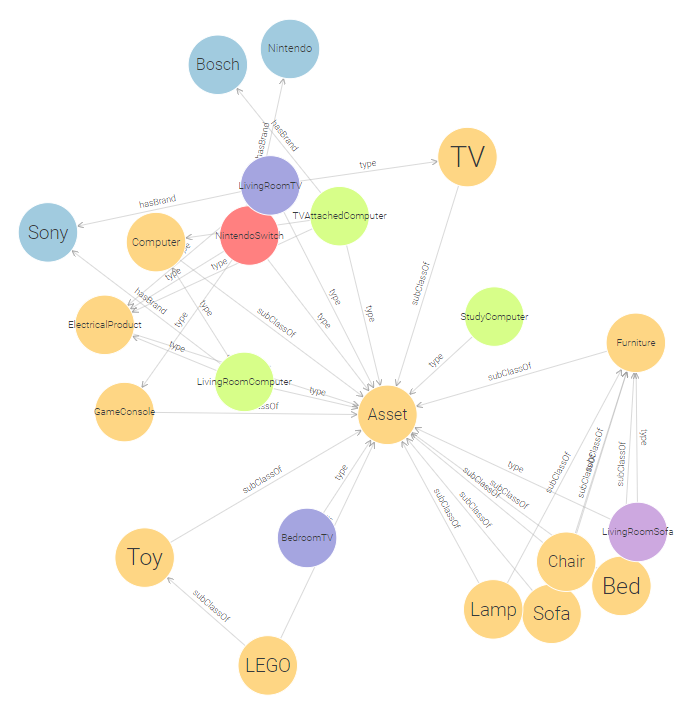
\includegraphics[width=\textwidth]{./chapters/ch-semanticwebpractice/figures/house_asset_exp.png}
	\caption{An example of an RDF model in GraphDB that describes house assets. This is only a demonstration graph and the information inside is artificial and not true.}
	\label{fig:houseassetexp}
\end{figure}

\subsection{Define Classes Hierarchy}

\subsection{Define Properties Hierarchy}

\subsection{Add OWL}

\subsection{Data Retrieval Examples}

\section{Reference: Commonly Used Namespace}

Commonly used built-in name spaces are summarized in Table \ref{tab:commonnamespace}.

\begin{table}
	\centering \caption{Commonly used name spaces in RDF models. URI is neglected since they can be easily found online.} \label{tab:commonnamespace}
	\begin{tabularx}{\textwidth}{lX}
		\hline
		Namespace & Description \\ \hline
		\verb|rdf| & RDF syntax. \\
		\verb|rdfs| & RDFS syntax. \\
		\verb|xsd|  & XML syntax. \\
		\verb|foaf| & Friend-of-a-friend. It describes people, their activities and relations to other people and object. \\
		\hline
	\end{tabularx}
\end{table}

To search URI for a name space, use \textit{prefix.cc}.





























